\subsection{应用举例}\label{subsec:15-6}
\begin{enhancedline}

解直角三角形的应用非常广泛,下面举一些例子。

\liti 厂房屋顶人字架(等腰三角形)的跨度为 $10$ 米,角 $A$ 为 $26^\circ$(图 \ref{fig:15-12})。
求中柱 $BC$($C$ 为底边中点)和上弦 $AB$ 的长(精确到 $0.01$ 米)。

\jie 由题意可知,$\triangle ABC$ 为直角三角形,其中 $C = 90^\circ$,$A = 26^\circ$,$AC = 5 \; \mi$。

$\because$   \quad $\tan A = \dfrac{BC}{AC}$,

$\therefore$ \quad $BC = AC \cdot \tan A = 5 \times \tan 26^\circ = 5 \times 0.4877 \approx 2.44 \; (\mi)$。

$\because$   \quad $\cos A = \dfrac{AC}{AB}$,

$\therefore$ \quad $AB = \dfrac{AC}{\cos A} = \dfrac{5}{\cos 26^\circ}$。

两边取对数,得

\hspace*{2em} $\lg{AB} = \lg{5} - \lg{\cos 26^\circ}$。

\hspace*{2em} \begin{tblr}[t]{
    columns={r, mode=math, colsep=0em},
    rows={rowsep=0em},
    hline{3}={1}{solid},
}
    \lg{5} = 0.6990 \\
    \lg{\cos 26^\circ} = \overline{1}.9537 \tikz [overlay] {\draw (1em, -0.5em) node {$(-$};} \\
    \lg{AB} = 0.7453
\end{tblr}

查反对数表得

\hspace*{2em} $AB = 5.563 \approx 5.56 \; (\mi)$。

答, $BC$ 约为 $2.44$ 米,$AB$ 约为 $5.56$ 米。


\begin{figure}[htbp]
    \centering
    \begin{minipage}[b]{6.5cm}
        \centering
        \begin{tikzpicture}[>=Stealth,
    every node/.style={fill=white, inner sep=1pt, outer sep=3pt},
]
    \pgfmathsetmacro{\b}{3}       % AC 的长度
    \pgfmathsetmacro{\jiaoa}{26}
    \pgfmathsetmacro{\a}{tan(\jiaoa) * \b}
    \pgfmathsetmacro{\c}{sqrt(\a*\a + \b*\b)}
    \pgfmathsetmacro{\r}{0.7}

    \coordinate (A) at (0, 0);
    \coordinate (B) at (\b, \a);
    \coordinate (C) at (\b, 0);
    \coordinate (D) at (2*\b, 0);

    \draw (A) node [left] {$A$} -- (C);
    \draw (C) node [below] {$C$} -- (B) node [midway, right==0.2em] {\small 中柱};
    \draw (B) node [above] {$B$} -- (A) node [midway, above, rotate=\jiaoa] {\small 上弦};
    \draw (0:\r) arc (0:\jiaoa:\r) node [pos=0.8, right=0.5em] {\footnotesize $\jiaoa^\circ$};

    \draw (B) -- (D) -- (C);
    % \draw [<->] ($(A) + (0, -0.7cm)$) to [xianduan={above=0.7cm}] node {\small 跨度} ($(D) + (0, -0.7cm)$);
    \draw [<->, transform canvas = {yshift=-0.7cm}] (A) to [xianduan={above=0.7cm}] node {\small 跨度} (D);
\end{tikzpicture}


        \caption{}\label{fig:15-12}
    \end{minipage}
    \qquad
    \begin{minipage}[b]{8cm}
        \centering
        \begin{tikzpicture}[
    every node/.style={fill=white, inner sep=1pt, outer sep=3pt},
]
% 各坐标点的相对位置
% H      A    D      K
%     B  E    F  C
%
% I                  J

    % 以 B 为原点,通过直角三角形 ABE 计算坐标
    \pgfmathsetmacro{\factor}{0.02}
    \pgfmathsetmacro{\jiaob}{55}
    \pgfmathsetmacro{\b}{70 * \factor}  % AE=70mm
    \pgfmathsetmacro{\a}{49 * \factor}  % BE=70mm
    \pgfmathsetmacro{\e}{sqrt(\a*\a + \b*\b)}
    \pgfmathsetmacro{\ad}{180 * \factor} % AD=180mm
    \pgfmathsetmacro{\x}{100 * \factor} % A 点扩展点 H 的水平间隔
    \pgfmathsetmacro{\y}{130 * \factor} % 扩展点 H 点扩展点 I 垂直间隔

    \coordinate (B) at (0,  0);
    \coordinate (A) at (\a, \b);
    \coordinate (E) at (\a, 0);
    \coordinate (F) at (\a + \ad, 0);
    \coordinate (C) at (\a + \ad + \a, 0);
    \coordinate (D) at (\a + \ad, \b);

    \coordinate (H) at ($(A) - (\x, 0)$);
    \coordinate (I) at ($(H) - (0, \y)$);
    \coordinate (K) at ($(D) + (\x, 0)$);
    \coordinate (J) at ($(K) - (0, \y)$);

    \draw [thick, pattern={mylines[angle=45, distance={5pt}]}]
        (H) -- (I) -- (J) -- (K)
            -- (D) -- (C) -- (B) -- (A) -- cycle;
    \draw [dashed] (A) -- (D);
    \draw (A) to[chuizu={direction=left}] (E);
    \draw (D) to[chuizu={direction=right}] (F);

    \node [above] at (A) {$A$};
    \node [left]  at (B) {$B$};
    \node [right] at (C) {$C$};
    \node [above] at (D) {$D$};
    \node [below] at (E) {$E$};
    \node [below] at (F) {$F$};
\end{tikzpicture}


        \caption{}\label{fig:15-13}
    \end{minipage}
\end{figure}


\begingroup
\renewcommand{\haomi}{\mathord{\text{mm}}}%毫米

\liti 燕尾槽的横断面是等腰梯形。图 \ref{fig:15-13} 是一燕尾槽的横断面,其中燕尾角 $B$ 是 $55^\circ$,
外口宽 $AD$ 是 $180\;\haomi$, 燕尾槽的深度是 $70\;\haomi$。
求它的里口宽 $BC$(精确到 $1\;\haomi$)。

分析:连结 $AD$,并分别作 $AE$,$DF$ 垂直于 $BC$,则 $AD = EF$,$BE = FC$。
又 $BC = BE + EF + FC = 2BE + AD$。由于 $AD$ 已知,只要求出 $BE$,这个问题就解决了。

\jie 作 $AE \perp BC$,$DF \perp BC$。在直角三角形 $ABE$ 中,

$\because$   \quad $\cot B = \dfrac{BE}{AE}$,

$\therefore$ \quad $BE = AE \cdot \cot B = 70 \times \cot 55^\circ = 70 \times 0.7002 \approx 49 \; (\haomi)$。

$\therefore$ \quad $BC = 2BE + AD \approx 2 \times 49.0 + 180 = 278 \; (\haomi)$。

答:燕尾槽的里口宽 $BC$ 约为 $278 \; \haomi$。
\endgroup


\liti 如图 \ref{fig:15-14},在山坡上种树,要求株距(两树间的水平距离)是 $5.5$ 米。
测得斜坡的倾斜角是 $24^\circ$,求斜坡上相邻两树间的倾斜距离是多少米(精确到 $0.1$ 米)。

\begin{figure}[htbp]
    \centering
    \begin{minipage}[b]{8cm}
        \centering
        %\input{../pic/czds4-ch15-14-1}
        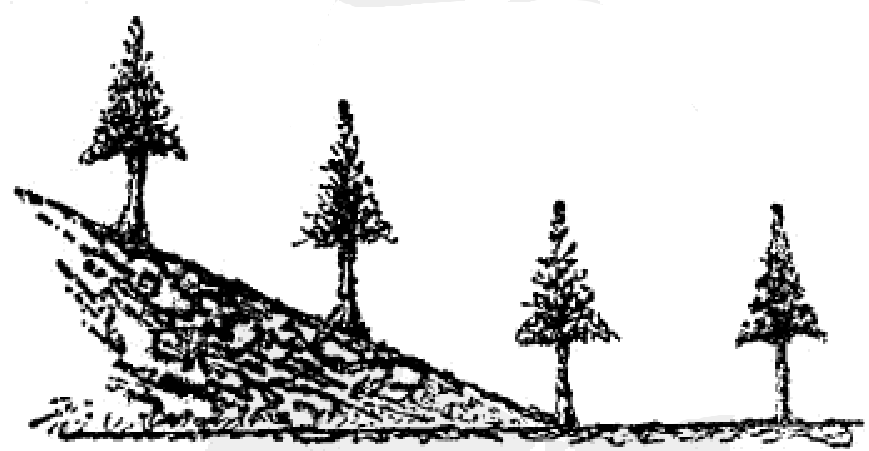
\includegraphics[width=0.6\textwidth]{../pic/czds4-ch15-14-1}
        \caption*{(1)}
    \end{minipage}
    \qquad
    \begin{minipage}[b]{6cm}
        \centering
        \begin{tikzpicture}[>=Stealth,
    every node/.style={fill=white, inner sep=1pt, outer sep=3pt},
]
    % 以 A 为原点
    \pgfmathsetmacro{\b}{3}       % 表示 5.5 米
    \pgfmathsetmacro{\jiaoa}{24}
    \pgfmathsetmacro{\a}{tan(\jiaoa) * \b}
    \pgfmathsetmacro{\c}{sqrt(\a*\a + \b*\b)}
    \pgfmathsetmacro{\r}{0.7}

    \coordinate (A) at (0, 0);
    \coordinate (B) at (-\b, \a);
    \coordinate (C) at (-\b, 0);

    \draw (A) -- ($(A)!1.3!(B)$);
    \draw (A) -- ($(A)!1.3!(C)$);
    \draw (180:\r) arc (180:180-\jiaoa:\r) node [pos=0.8, left=0.5em] {\small $\jiaoa^\circ$};
    \draw (A) -- ($(A) + (0, 0.5)$);
    \draw (B) -- ($(B)!-0.3!(C)$);
    \draw [dashed] (B) -- (C);
    \draw (B) to [chuizu={skipline=true}] (C);
    %\draw (C) rectangle ($(C) + (0.2, 0.2)$);
    \node [right] at (A) {$A$};
    \node [above right] at (B) {$B$};
    \node [below left]  at (C) {$C$};
    %\draw [<->] ($(C) + (0, -1em)$) to [xianduan={above=1em}] node {\small $5.5$ 米} ($(A) + (0, -1em)$);
    \draw [<->, transform canvas = {yshift=-1em}] (C) to [xianduan={above=1em}] node {\small $5.5$ 米} (A);
\end{tikzpicture}


        \caption*{(2)}
    \end{minipage}
    \caption{}\label{fig:15-14}
\end{figure}


分析:如图 \ref{fig:15-14} (2), $\angle A = 24^\circ$,水平距离 $AC = 5.5$米,$BC \perp AC$,
$\triangle ABC$ 是直角三角形。只要解 $\triangle ABC$ 求出 $AB$,问题就解决了。

\jie 在 $\triangle ABC$ 中, $\angle C = 90^\circ$,

\hspace*{3em} \begin{tblr}{rows={rowsep=0.5em, mode=math}}
    \cos A = \dfrac{AC}{AB} \douhao \\
    AB = \dfrac{AC}{\cos A} = \dfrac{5.5}{0.9135} \approx 6.0 \; (\mi) \juhao
\end{tblr}

答:斜坡上相邻两树间的倾斜距离约是 $6.0$ 米。

\begin{wrapfigure}[7]{r}{7.5cm}
    \centering
    \begin{tikzpicture}[>=Stealth,
    every node/.style={fill=white, inner sep=1pt, outer sep=3pt},
    scale=0.8,
]
% 各坐标点 (A-G) 的相对位置
%       C    D
% A  B       |
%            E   F  G
    \coordinate (A) at (0, 0);
    \coordinate (B) at ($(A) + (1, 0)$);
    \coordinate (C) at ($(B) + (2, 2)$);
    \coordinate (D) at ($(C) + (2, 0)$);
    \coordinate (E) at ($(D) - (0, 3)$);
    \coordinate (F) at ($(E) + (3, 0)$);
    \coordinate (G) at ($(F) + (1, 0)$);

    \draw (A) -- (B) -- (C) -- (D)  -- (F) -- (G);
    \draw [dashed] (D) -- (E) -- (F);
    \draw (D) to [chuizu={skipline=true}] (E);
    % \draw [<->] ($(E) + (0, -1em)$) to [xianduan={above=1em}] node {$l$} ($(F) + (0, -1em)$);
    % \draw [<->] ($(E) + (-1em, 0)$) to [xianduan={below=1em}] node [rotate=90] {$h$} ($(D) + (-1em, 0)$);
    \draw [<->, transform canvas = {yshift=-1em}] (E) to [xianduan={above=1em}] node {$l$} (F);
    \draw [<->, transform canvas = {xshift=-1em}] (E) to [xianduan={below=1em}] node [rotate=90] {$h$} (D);
    \draw (D) -- (F) node [midway, above, rotate=-45] {$i = h : l$};

    \pgfmathsetmacro{\r}{0.7}
    \draw (F) + (180:\r)  arc (180:135:\r);

    \coordinate (X) at ($(F) + (0.5, 1.2)$);
    \path [path picture={\draw (path picture bounding box.north west) pic {waterwave};}]
        (X) -- ($(X) + (-1.4, 0.7)$) -- ($(X) + (0.8, 0.7)$) -- cycle;
\end{tikzpicture}


    \caption{}\label{fig:15-15}
\end{wrapfigure}

在筑坝、开渠、挖河和修路时,设计图纸上都要注明斜坡的倾斜程度。
通常把坡面的铅直高度 $h$ 和水平宽度 $l$ 的比叫做\zhongdian{坡度}
(或叫做\zhongdian{坡比})(图 \ref{fig:15-15}),用字母 $i$ 表示,即
$$ i = \exdfrac{h}{l} \juhao $$
坡度一般写成 $1:m$ 的形式,如 $i = 1:5 \left(\text{即 \;} i = \exdfrac{1}{5} \right)$。

如果把坡面与水平面的夹角记作 $\alpha$(叫做\zhongdian{坡角}),那么
$$ i = \exdfrac{h}{l} = \tan \alpha \juhao $$
显然,坡度越大(于是 $\alpha$ 角越大),坡面就越陡。


\begingroup
\renewcommand{\mi}{\mathord{\text{m}}}%米

\liti 水库大坝的横断面是梯形(图 \ref{fig:15-16}),坝顶宽 $6 \;\mi$,坝高 $23 \; \mi$,
斜坡 $AB$ 的坡度 $i = 1:3$,斜坡 $CD$ 的坡度 $i' = 1:2.5$。
求斜坡 $AB$ 的坡角 $\alpha$,坝底宽 $AD$ 和斜坡 $AB$ 的长(精确到 $0.1 \; \mi$)。

\begin{figure}[htbp]
    \centering
    \begin{tikzpicture}
    \pgfmathsetmacro{\r}{0.5}
    \pgfmathsetmacro{\a}{2.3}
    \pgfmathsetmacro{\e}{3 * \a}
    \pgfmathsetmacro{\b}{sqrt(\e*\e - \a*\a)}
    \pgfmathsetmacro{\jiaoa}{asin(\a/\e)}
    \pgfmathsetmacro{\d}{\a}
    \pgfmathsetmacro{\f}{2.5 * \a}
    \pgfmathsetmacro{\c}{sqrt(\f*\f - \d*\d)}
    \pgfmathsetmacro{\jiaod}{asin(\d/\f)}

    \coordinate (A) at (0, 0);
    \coordinate (B) at (\b, \a);
    \coordinate (E) at (\b, 0);
    \coordinate (C) at ($(B) + (0.6, 0)$);
    \coordinate (F) at ($(E) + (0.6, 0)$);
    \coordinate (D) at ($(F) + (\c, 0)$);

    \draw (A) -- (B) node [midway, above, rotate=\jiaoa] {$1:3$};
    \draw (B) -- (C) node [midway, above] {\small $6$m};
    \draw (C) -- (D) node [midway, above, rotate=-\jiaod] {$1:2.5$};
    \draw (A) -- (D);
    \draw [dashed] (B) -- (E) node [midway, above, rotate=90] {\small $23$m};
    \draw [dashed] (C) -- (F);
    \draw (B) to [chuizu={skipline=true}] (E);
    \draw (C) to [chuizu={skipline=true}] (F);

    \draw (B) node [above left]  {$B$};
    \draw (C) node [above right] {$C$};
    \foreach \x in {A, E, F, D} {
        \draw (\x) node [below] {$\x$};
    }
\end{tikzpicture}


    \caption{}\label{fig:15-16}
\end{figure}

\jie 在图 \ref{fig:15-16} 中,作 $BE \perp AD$,$CF \perp AD$。在直角三角形 $ABE$ 和 $CDF$ 中,

$\because$   \quad $\dfrac{BE}{AE} = 1:3$,$\dfrac{CF}{FD} = 1:2.5$,

$\therefore$ \quad $AE = 3BE = 3 \times 23 = 69 \; (\mi)$,

\hspace*{2em}$FD = 2.5CF = 2.5 \times 23 = 57.5 \; (\mi)$。

$\therefore$ \quad $AD = AE + EF + FD = 69 + 6 + 57.5 = 132.5 \; (\mi)$。

因为斜坡 $AB$ 的坡度 $i = \tan \alpha = \exdfrac{1}{3} \approx 0.3333$,查表得
$$ \alpha \approx 18^\circ26' \juhao $$

$\because$   \quad $\dfrac{BE}{AB} = \sin \alpha$,

$\therefore$ \quad $AB = \dfrac{BE}{\sin \alpha} = \dfrac{23}{\sin 18^\circ26'} = 72.73 \approx 72.7 \; (\mi)$。

答:斜坡 $AB$ 的坡角 $\alpha$ 约为 $18^\circ26'$,坝底宽 $AD$ 为 $132.5$ 米,斜坡 $AB$ 的长约为 $72.7$ 米。

在例 4 中,也可由 $\dfrac{BE}{AE} = 1:3$, 得 $\dfrac{BE}{AB} = 1:\sqrt{10}$,求得
$$ AB = \sqrt{10} \cdot BE = \sqrt{10} \times 23 \approx 72.7 \; (\mi) \juhao $$
\endgroup
\end{enhancedline}


\lianxi
\begin{xiaotis}

\xiaoti{如图,某厂车间的人字屋架为等腰三角形,跨度 $AB = 12$ 米,$\angle A = 22^\circ$,
    求中柱 $CD$ 和上弦 $AC$ 的长(精确到 $0.01$ 米)。
}

\begin{figure}[htbp]
    \centering
    \begin{minipage}[b]{8cm}
        \centering
        \begin{tikzpicture}
    \pgfmathsetmacro{\c}{3} % 用 3 表示 12/2
    \pgfmathsetmacro{\jiaoa}{22}
    \pgfmathsetmacro{\a}{\c * tan(\jiaoa)}

    \coordinate (A) at (0, 0);
    \coordinate (C) at (\c, \a);
    \coordinate (D) at (\c, 0);
    \coordinate (B) at (2*\c, 0);

    \coordinate (AC1) at ($(A)!0.33!(C)$);
    \coordinate (AC2) at ($(A)!0.66!(C)$);
    \coordinate (BC1) at ($(B)!0.33!(C)$);
    \coordinate (BC2) at ($(B)!0.66!(C)$);

    \draw (A) node [left] {$A$} -- (B) node [right] {$B$} -- (C) node [above] {$C$} --cycle;
    \draw (C) -- (D) node [below] {$D$};
    \draw (D) -- (AC2) -- (AC2 |- A) -- (AC1) -- (AC1 |- A);
    \draw (D) -- (BC2) -- (BC2 |- A) -- (BC1) -- (BC1 |- A);
\end{tikzpicture}


        \caption*{(第 1 题)}
    \end{minipage}
    \qquad
    \begin{minipage}[b]{6cm}
        \centering
        \begin{tikzpicture}[>=Stealth]
    \pgfmathsetmacro{\r}{0.3}
    \pgfmathsetmacro{\p}{0.08}
    \pgfmathsetmacro{\a}{2}
    \pgfmathsetmacro{\jiaoa}{60}
    \pgfmathsetmacro{\c}{\a * cot(\jiaoa)}

    \coordinate (A) at (-\c - \p, 0);
    \coordinate (C1) at (-\p, \a);
    \coordinate (D1) at (-\p, 0);
    \coordinate (B) at (\c + \p, 0);
    \coordinate (C2) at (\p, \a);
    \coordinate (D2) at (\p, 0);

    \draw (A) node [below=0.6em] {$A$} -- (C1) node [left] {$C$} -- (D1) node [below=0.6em] {$D$} -- cycle;
    \draw (A) + (0:\r) arc (0:\jiaoa:\r) node [midway, above right] {\small $\jiaoa^\circ$};
    \draw (B) node [below=0.6em] {$B$} -- (C2) -- (D2) -- cycle;
    \draw (D1) rectangle ($(D1) + (2*\p, 3.5)$);
    \draw [ground={angle=-135}, name path=gnd] [thick] (-2, 0) -- (2, 0);
    \draw [<->] (1.6, 0) to [xianduan={above=1.5cm}] node [above, rotate=90] {$5$m} (1.6, \a);
    \draw [fill=black] ($(C1) - (\p, \p/2)$) rectangle ($(C1) + (3*\p, \p/2)$);

    \begin{scope}[yshift=2.5cm]
        \pgfmathsetmacro{\len}{6*\p}
        \draw [fill=black] (-\len/2, 0) rectangle (\len/2, \p);
        \foreach \x in {-4, ..., 4} {
            \draw (\len*\x/10,\p)  -- +(0, 0.06);
        }
    \end{scope}

    \begin{scope}[yshift=3.1cm]
        \draw (-4*\p, 0) rectangle (4*\p, \p);
        \foreach \x in {-4, ..., 4} {
            \draw (8*\p*\x/10,\p)  -- +(0, 0.06);
        }
    \end{scope}
\end{tikzpicture}


        \caption*{(第 2 题)}
    \end{minipage}
\end{figure}


\xiaoti{如图,在离地面高 $5$ 米处引拉线固定电线杆,拉线和地面成 $60^\circ$ 角,求拉线 $AC$ 的长,
    拉线下端点 $A$ 离杆底 $D$ 多远(精确到 $0.01$ 米)。
}

\xiaoti{如图,沿 $AC$ 方向开山修渠,为了加快施工进度,要在小山的另一边同时施工。
    从 $AC$ 上的一点 $B$ 取 $\angle ABD = 140^\circ$,$BD = 520 \; \mi$,$\angle D = 50^\circ$,
    那么开挖点 $E$ 离 $D$ 多远(精确到 $0.1$ 米),才能使 $A$,$C$,$E$ 成一直线?
}

\begin{figure}[htbp]
    \centering
    \begin{minipage}[b]{7cm}
        \centering
        \begin{tikzpicture}
    \coordinate (A) at (0, 0);
    \coordinate (B) at (2, 0);
    \coordinate (C) at (3, 0);
    \coordinate (D) at ($(B) + (320:5)$);

    \draw (A) node [above] {$A$}
        -- (B) node [above] {$B$}
        -- (C) node [above] {$C$};
    \draw (B) -- (D) node [right] {$D$};
    \path [name path=p1] (A) -- +(6, 0);
    \path [name path=p2] (D) -- +(90:4);
    \draw [name intersections={of=p1 and p2, by=E}]
        (D) -- (E) node [right] {$E$};

    \pgfmathsetmacro{\r}{0.5}
    \draw (B) + (180:\r) arc (180:320:\r) node [midway, below left] {\small $140^\circ$};
    \draw (D) + (90:\r) arc (90:140:\r) node [pos=0.7, above] {\small $50^\circ$};

    \pic [scale=0.1] at (4.4, -1.5) {mountain};
\end{tikzpicture}


        \caption*{(第 3 题)}
    \end{minipage}
    \qquad
    \begin{minipage}[b]{8cm}
        \centering
        \begin{tikzpicture}[>=Stealth,
    every node/.style={fill=white, inner sep=1pt, outer sep=3pt},
]
    \pgfmathsetmacro{\factor}{0.3}
    \pgfmathsetmacro{\a}{5.8 * \factor}
    \pgfmathsetmacro{\e}{\a * 1.6}
    \pgfmathsetmacro{\jiaoa}{asin(\a/\e)}
    \pgfmathsetmacro{\b}{cos(\jiaoa) * \e}
    \pgfmathsetmacro{\r}{0.5}

    \coordinate (A) at (0, 0);
    \coordinate (B) at (\b ,\a);
    \coordinate (C) at ($(B) + (9.8 * \factor, 0)$);
    \coordinate (D) at (2 * \b + 9.8 * \factor, 0);

    \fill [draw, thick, pattern = dots]
            (A) node [below] {$A$}
         -- (B) node [above left] {$B$} node [midway, above, rotate=\jiaoa] {$i = 1:1.6$}
         -- (C) node [above right] {$C$}
         -- (D) node [below] {$D$}
         -- cycle;
    \draw (A)  + (0:\r) arc (0:\jiaoa:\r) node [pos=0.8, right] {$\alpha$};
    \draw [<->, transform canvas = {yshift=0.5em}] (B) to [xianduan] node [above] {$9.8$m} (C);
    \draw [<->, transform canvas = {xshift=0.5em}] (D) to [xianduan={above=\b cm + 0.5em}] node [above, rotate=90] {$5.8$m} ($(D) + (0, \a)$);
\end{tikzpicture}


        \caption*{(第 4 题)}
    \end{minipage}
\end{figure}

\xiaoti{如图,一铁路路基的横断面为等腰梯形 $ABCD$,
    根据图示数据计算出路基下底宽 $AD$(精确到 $0.1$ 米)和坡角 $\alpha$。
}

\end{xiaotis}

